\documentclass[11pt,a4j]{jsarticle}

\usepackage{float,array,booktabs,here}
\usepackage{amsmath}
\usepackage[dvipdfmx]{graphicx}
\usepackage[top=20truemm,bottom=25truemm,left=20truemm,right=20truemm]{geometry}
\usepackage{url}
\usepackage{listings, jlisting}

\lstset{language=c,
  frame=single,
  stepnumber=1,
  numbersep=2pt,
  tabsize=2,
  basicstyle=\verysmall\ttfamily,
  stringstyle=\small\texttt,
  commentstyle=\slshape,
  captionpos=b,
  columns=[l]{fullflexible}
}

\makeatletter
\newcommand{\figcaption}[1]{\def\@captype{figure}\caption{#1}}
\newcommand{\tblcaption}[1]{\def\@captype{table}\caption{#1}}
\makeatother

\newcommand{\Maru}[1]{\ooalign{
\ifnum#1<10 \hfil\resizebox{.9\width}{.85\height}{#1}\hfil
\else
\hfil\resizebox{.6\width}{.8\height}{#1}\hfil
\fi
\crcr
\raise.1ex\hbox{$\bigcirc$}}}


\begin{document}

\input{title}


\section{外部仕様}
\label{sec:外部仕様}

\subsection{概要}
\label{sub:概要}

モグラ叩きゲームを作成した。
難易度は3種類あり、選択してからゲームをスタートする。
制限時間は20秒であり、ゲーム終了後に3位までのハイスコアが表示される。
プレーヤーが3位までのスコアを上回った場合、メッセージが表示される。

\subsection{実験装置}
\label{sub:実験装置}
実験に使用したFPGAボードと液晶モニタ、拡張ボードを図\ref{fig:machine}に示す。

\begin{figure}[H]
  \centering
  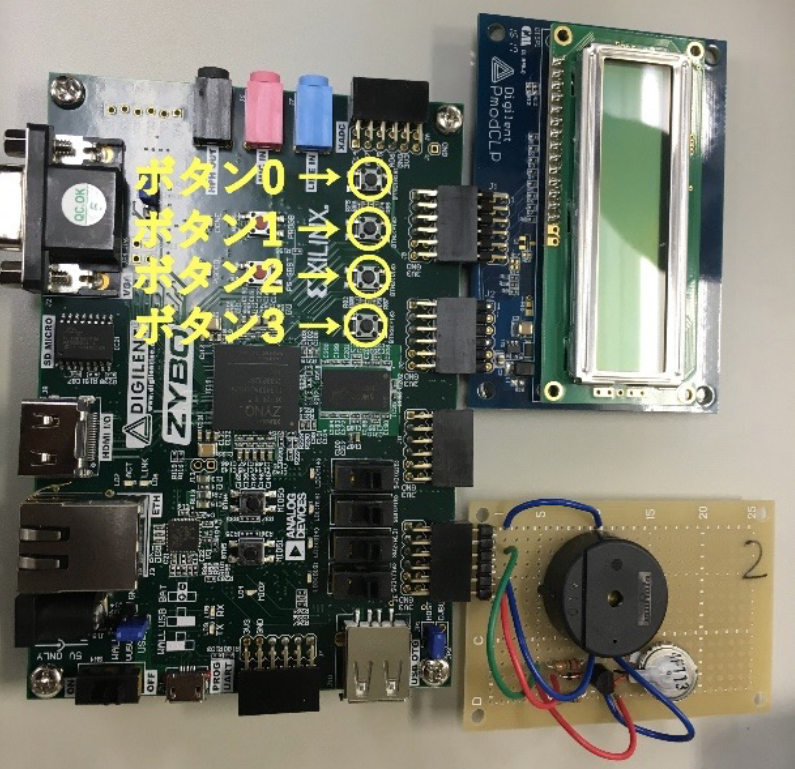
\includegraphics[height=60mm,bb=0 0 795 769]{img/machine.png}
  \figcaption{実験装置}
  \label{fig:machine}
\end{figure}

ゲームに使用するボタンを図\ref{fig:machine}のようにボタン0~3とした。

\subsection{ゲームの進め方}
\label{sub:ゲームの進め方}

まず、図\ref{fig:start}のようなスタート画面が表示される。

\begin{table}[H]
	\begin{center}
	\begin{tabular}{cc}
	\begin{minipage}{0.49\hsize}
    \centering
    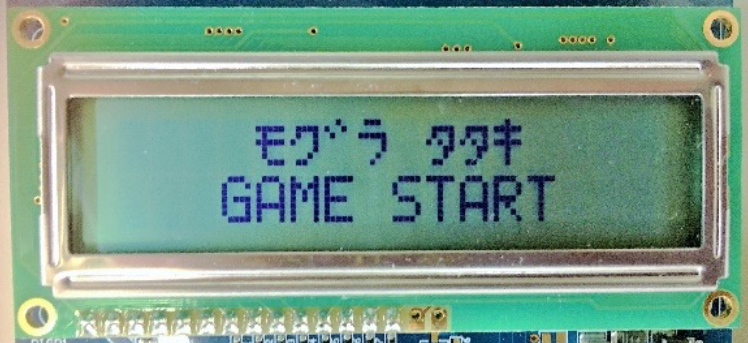
\includegraphics[height=25mm,bb=0 0 748 343]{img/start.png}
    \figcaption{スタート画面}
    \label{fig:start}
	\end{minipage} &
	\begin{minipage}{0.49\hsize}
    \centering
    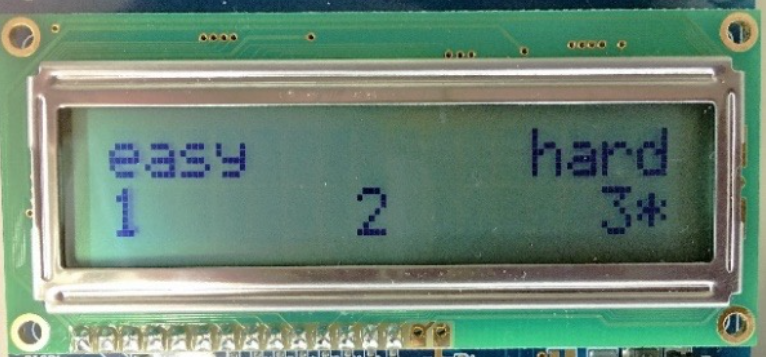
\includegraphics[height=25mm,bb=0 0 748 343]{img/select_mode.png}
    \figcaption{難易度選択画面}
    \label{fig:select}
	\end{minipage} \\
	\end{tabular}
	\end{center}
\end{table}


次に難易度を図\ref{fig:select}のように、3種類から選択する。


モード1が最も容易であり、モード3が最も難しい。
ボタン0でカーソルを左に、ボタン2でカーソルを右に移動する。
ボタン1で決定するとゲームがスタートする。



\begin{table}[H]
	\begin{center}
	\begin{tabular}{cc}
	\begin{minipage}{0.49\hsize}
    \centering
    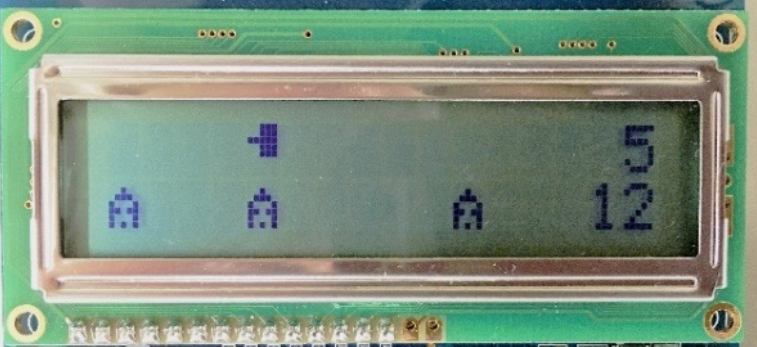
\includegraphics[height=25mm,bb=0 0 757 347]{img/play.png}
    \figcaption{プレイ画面}
    \label{fig:play}
	\end{minipage} &
	\begin{minipage}{0.49\hsize}
    \centering
    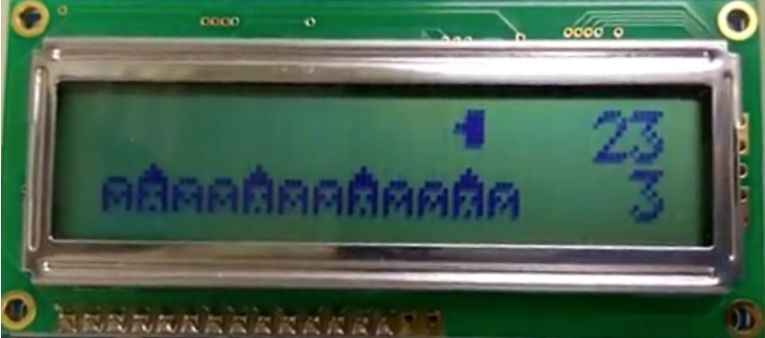
\includegraphics[height=25mm,bb=0 0 765 338]{img/feaver.png}
    \figcaption{フィーバータイム}
    \label{fig:feaver}
	\end{minipage} \\
	\end{tabular}
	\end{center}
\end{table}

図\ref{fig:play}はゲーム中の画面である。
制限時間は20秒であり、画面右上にはスコアが、右下には残り時間が表示されている。
ボタン0でハンマーを左に、ボタン2でハンマーを右に移動し、ボタン1でモグラを叩く。
モグラを叩くとスコアが1ずつ増えていき、ブザーが鳴る。ミスした場合モータが振動するが、スコアは変化しない。


残り時間3秒になった時にスコアが15以上であると、フィーバータイムとなり図\ref{fig:feaver}のようにボスモグラが出現する。
ボスモグラ出現時はハンマーがどこの位置にあってもボタン1を押すことでスコアを増やすことができる。


\begin{table}[H]
	\begin{center}
	\begin{tabular}{cc}
	\begin{minipage}{0.49\hsize}
    \centering
    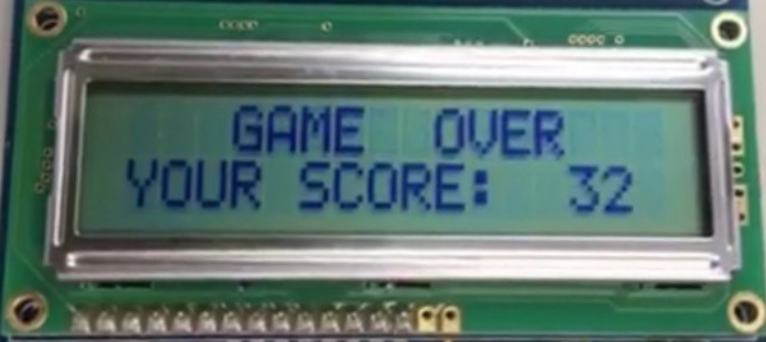
\includegraphics[height=25mm,bb=0 0 766 342]{img/result.png}
    \figcaption{結果の表示}
    \label{fig:result}
	\end{minipage} &
	\begin{minipage}{0.49\hsize}
    \centering
    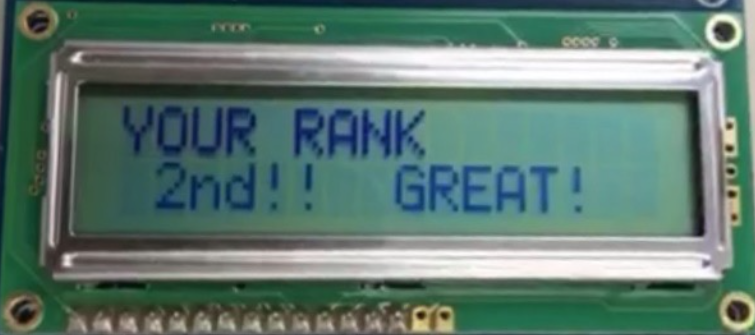
\includegraphics[height=25mm,bb=0 0 755 335]{img/update.png}
    \figcaption{ランキングの更新の表示}
    \label{fig:update}
	\end{minipage} \\
	\end{tabular}
	\end{center}
\end{table}

% \begin{figure}[H]
%   \centering
%   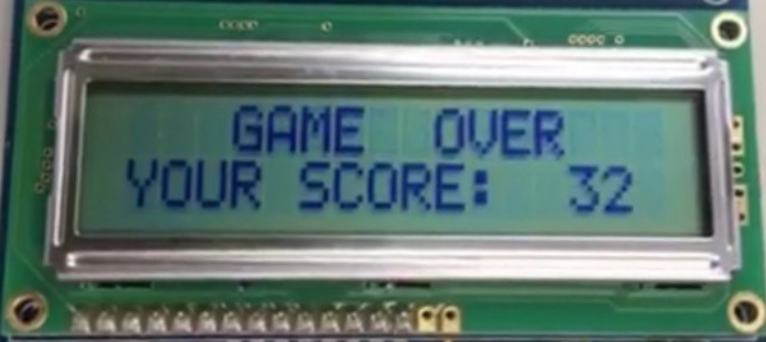
\includegraphics[height=25mm,bb=0 0 766 342]{img/result.png}
%   \figcaption{結果の表示}
%   \label{fig:result}
% \end{figure}
%
% \begin{figure}[H]
%   \centering
%   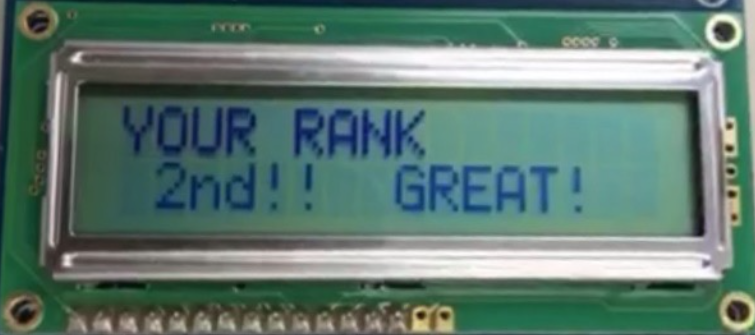
\includegraphics[height=25mm,bb=0 0 755 335]{img/update.png}
%   \figcaption{ランキングの更新の表示}
%   \label{fig:update}
% \end{figure}

残り時間が0になるとゲームが終了し、図\ref{fig:result}のようにスコアが表示される。
スコアが3位までのハイスコアを上回っている場合、図\ref{fig:update}のようにメッセージが表示される。

\begin{table}[H]
	\begin{center}
	\begin{tabular}{cc}
	\begin{minipage}{0.49\hsize}
    \centering
    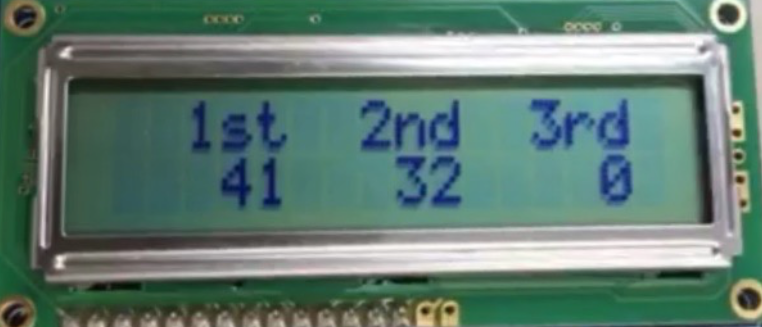
\includegraphics[height=25mm,bb=0 0 762 327]{img/ranking.png}
    \figcaption{ランキングの表示}
    \label{fig:ranking}
	\end{minipage} &
	\begin{minipage}{0.49\hsize}
    \centering
    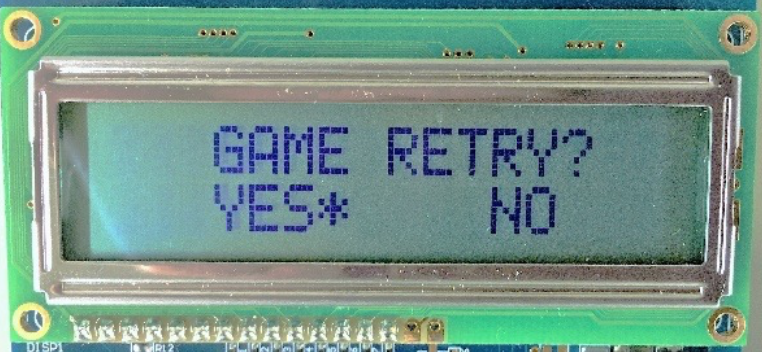
\includegraphics[height=25mm,bb=0 0 762 352]{img/retry.png}
    \figcaption{リトライの確認}
    \label{fig:retry}
	\end{minipage} \\
	\end{tabular}
	\end{center}
\end{table}



その後、図\ref{fig:ranking}のように3位までのスコアのランキングが表示される。


最後にリトライするかどうかの選択画面が表示される。
ボタン0とボタン2を用いてカーソルを動かし、ボタン1で決定する。
YESを選択すると同じモードでリトライすることができ、再びプレイ画面が表示される。


\section{内部仕様}
\label{sec:内部仕様}

\subsection{概要}
\label{sub:概要}

内部仕様は以下のようなフローチャートで表される。
紙面のサイズの都合により、切り出した形のフローチャートとなっている。

このアクティビティー図はplantUMLを用いて自分が作成した。

自分が担当したのは、図\ref{fig:flow2}と図\ref{fig:flow3}のプレイからリトライまでの部分である。

キャラクターのデザインや、アニメーションのアイデア、velilogのコードなどに関しては
他のメンバーに担当してもらって、自分はゲームのコードに専念させていただいた。

アニメーション表示のラッパー関数的なものも用意した。

\subsection{フローチャート}
\label{sub:フローチャート}


\begin{figure}[H]
  \centering
  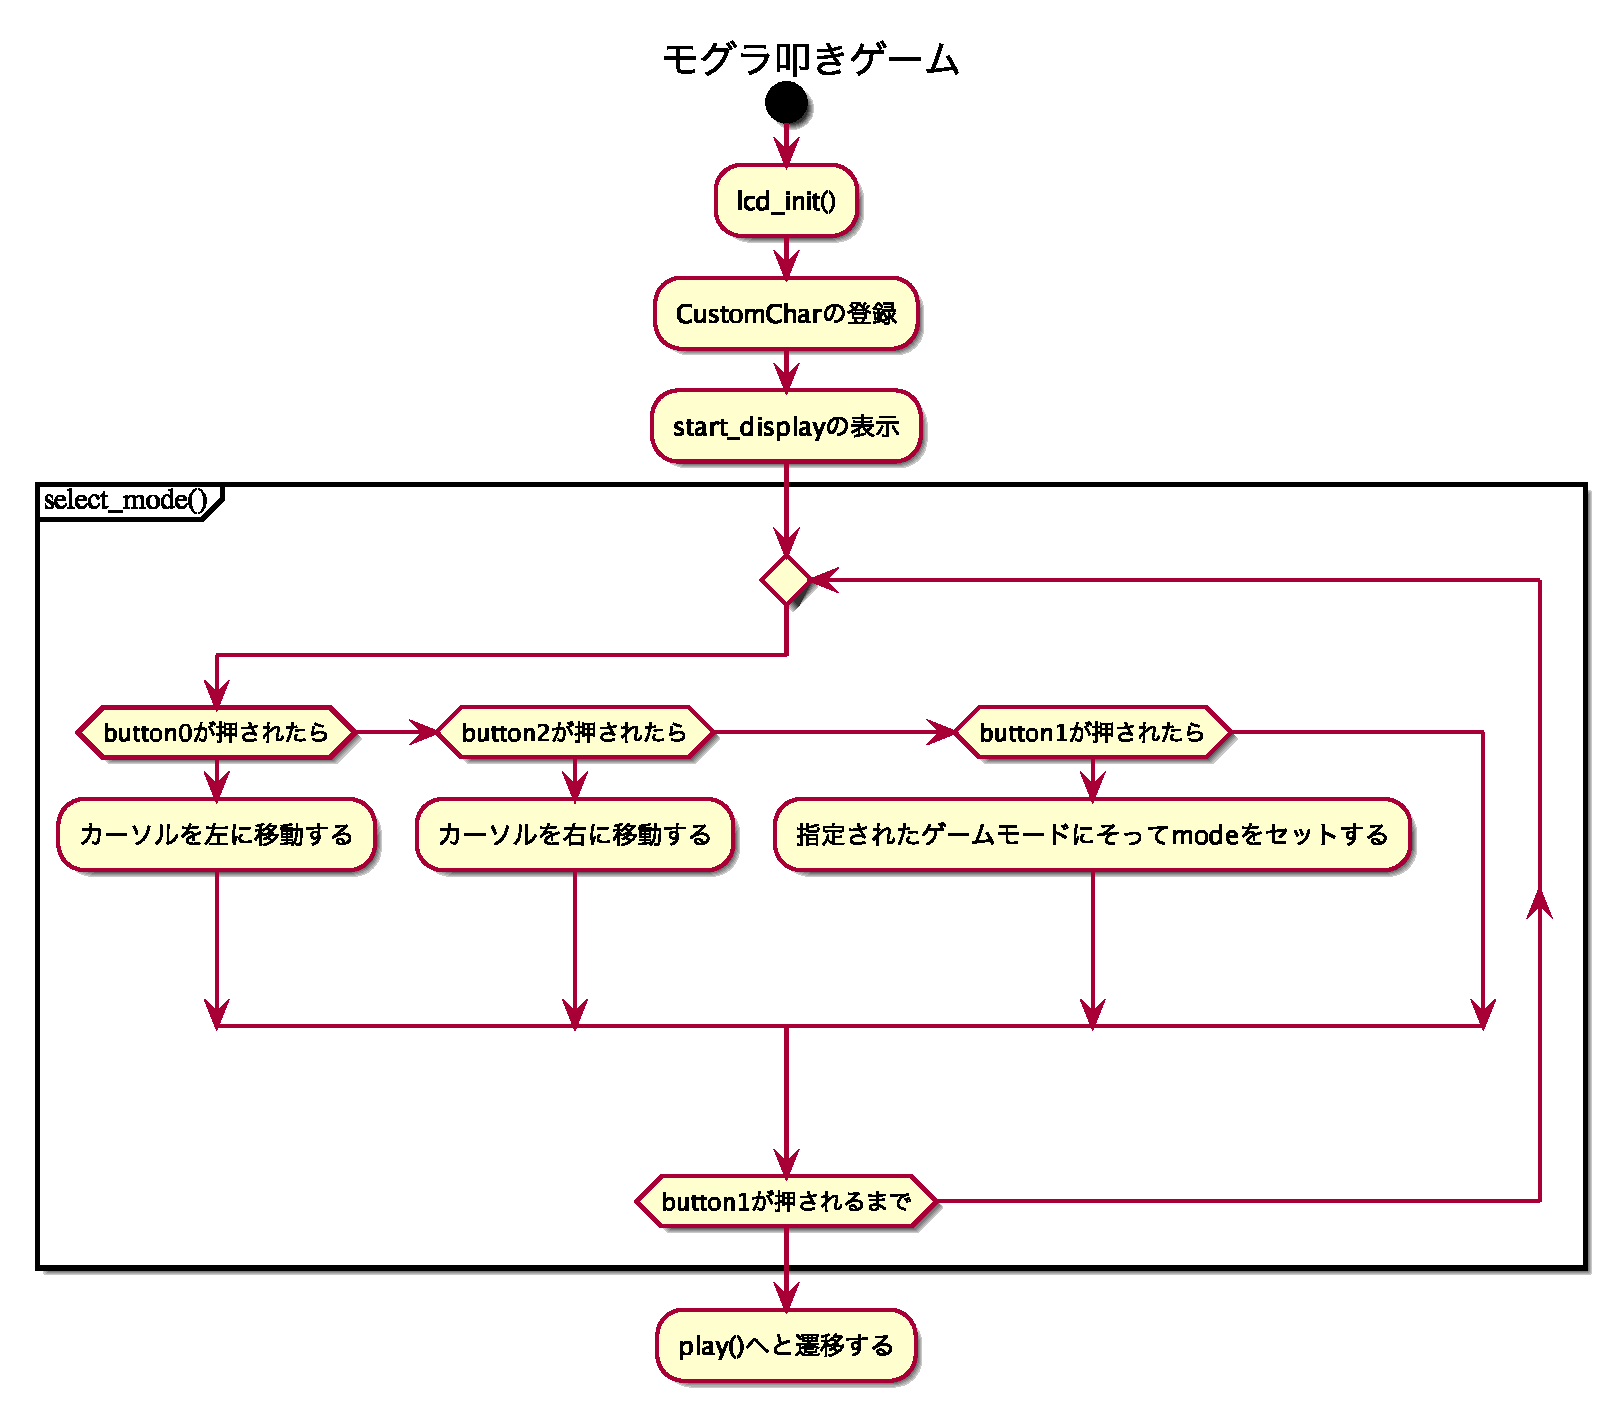
\includegraphics[height=70mm]{img/mogura_init.eps}
  \figcaption{内部仕様のフローチャート(難易度を選ぶまで)}
  \label{fig:flow1}
\end{figure}

\begin{figure}[H]
  \centering
  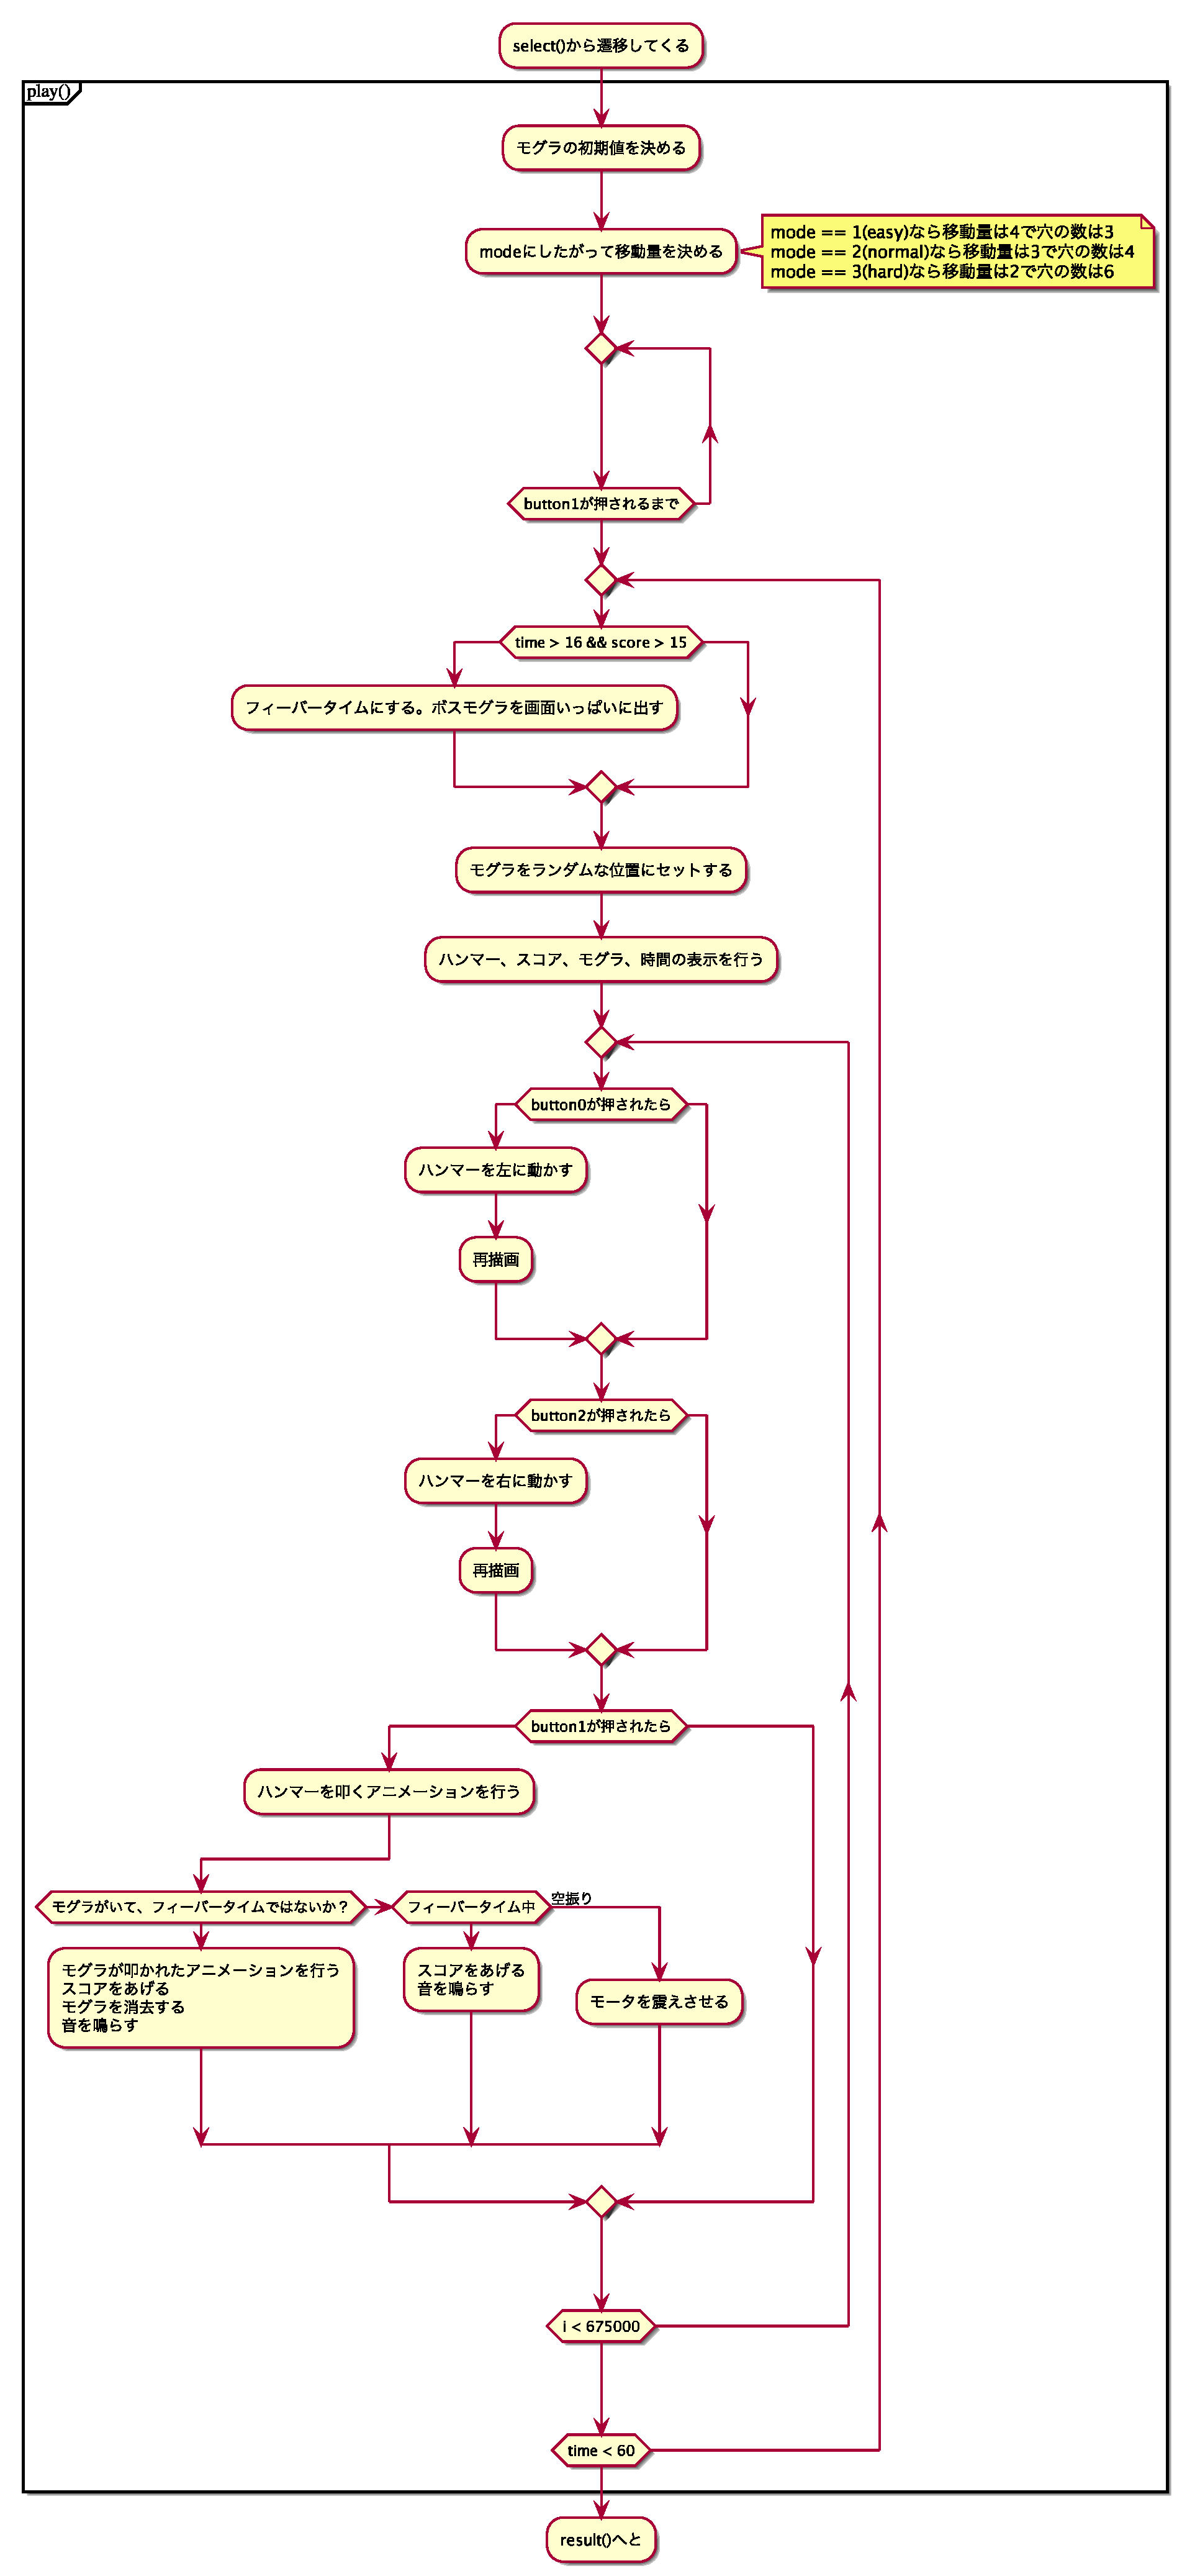
\includegraphics[height=225mm]{img/mogura_play.eps}
  \figcaption{内部仕様のフローチャート(プレイ画面)}
  \label{fig:flow2}
\end{figure}

\begin{figure}[H]
  \centering
  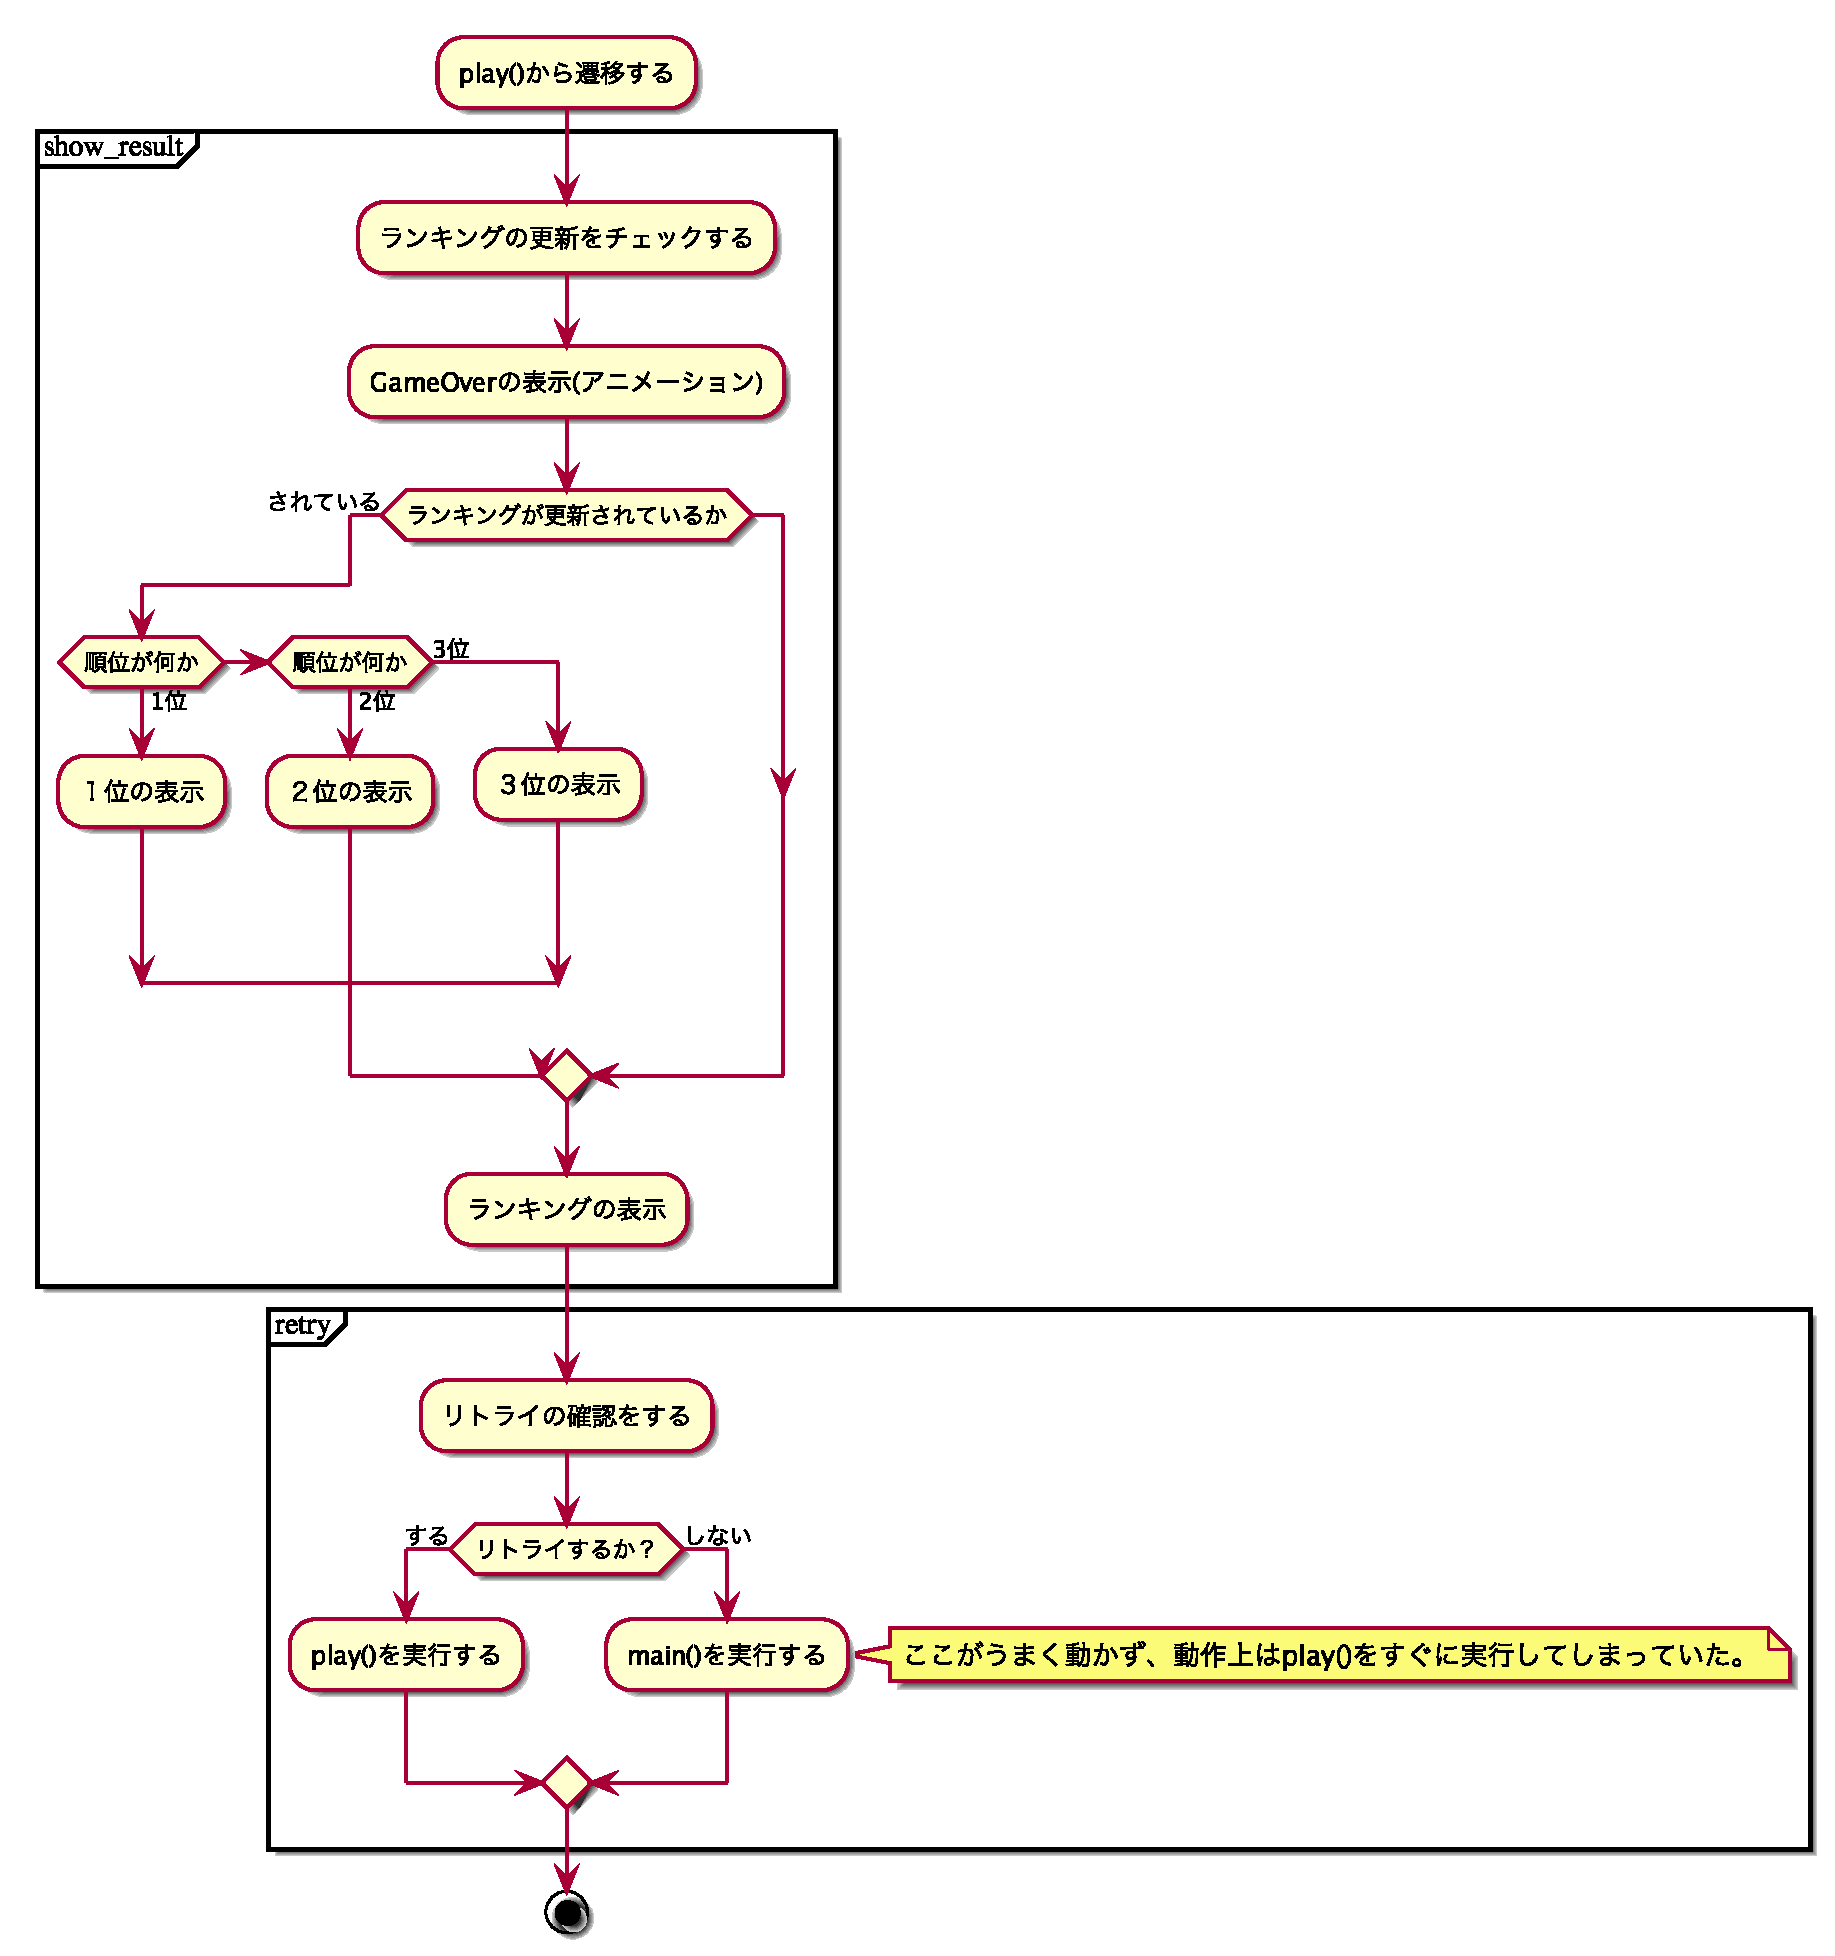
\includegraphics[height=100mm]{img/mogura_result.eps}
  \figcaption{内部仕様のフローチャート(結果表示とリトライ確認)}
  \label{fig:flow3}
\end{figure}

\subsection{コードに関して}
\label{sub:コードに関して}

実際に書いたコードに関して自分が書いたコードの中で主なものを解説していく。

\subsubsection{xorshiftでの乱数発生}
\label{subs:xorshiftでの乱数発生}

今回は、モグラがランダムに出現するようにするため、擬似乱数を使う必要があった。
そこで、最初は線形合同法にて実装を試みたが、浮動小数点を用いることができなかった為xorshiftでの実装を行った。
xorshiftの利点は、整数のxorとshiftしか扱わず非常に高速な計算が可能なところである。
少しの偏りはあるのだが、分布にこだわるのであればメルセンヌツイスター、
速度にこだわるのであればxorshiftを用いればいいのではないかと思った。

\begin{lstlisting}[basicstyle=\ttfamily\footnotesize, caption=xorshiftでの擬似乱数]
unsigned long xor128(){
	unsigned long t;
	t=(x^(x<<11));
	x=y;
	y=z;
	z=w;
	return( w=(w^(w>>19))^(t^(t>>8)) );
}

unsigned int xor32() {
	unsigned int x;
	x = xor128();
	return x;
}
\end{lstlisting}

\subsubsection{文字のanimationについて}
\label{subs:文字のanimationについて}

テキストの中にアニメーションさせる関数が用意されていたのに気づかず、異なった方法で実装を行った。
右端から、画面中央まで流す部分 \verb|(lcd_left_flow_before)| は動いたのだが、
画面中央から左端に流していく部分 \verb|(lcd_left_flow_after)| はメモリを破壊しているようで
うまく動かすことができなかった。

\begin{lstlisting}[basicstyle=\ttfamily\footnotesize, frame=single]
void lcd_left_flow_before(unsigned char *str1, unsigned char *str2)
{
	int i;
	for(i=0; i < 16; i++) {
		lcd_cmd(0x01);
		lcd_cmd(0x80 + 15 - i);
		lcd_str(str1);
		lcd_cmd(0xc0 + 15 - i);
		lcd_str(str2);
		lcd_wait(500000);
	}
}

void lcd_left_flow_after(unsigned char *str1, unsigned char *str2)
{
	int i;
	for(i = 0; i < 16 ; i++) {
		while (*str1 != 0x00) {
			lcd_cmd(0x01);
			lcd_cmd(0x80);
			lcd_str(str1);
			lcd_cmd(0xc0);
			lcd_str(str2);
		}
		lcd_wait(500000);
		int j;
		for(j=0;j<16;j++){
			str1[j] = str1[j+1];
			if(str1[j+1] == 0x00)
				break;
		}
	}
}
\end{lstlisting}

\subsubsection{ハンマーの移動について}
\label{subs:ハンマーの移動について}

play()の中でハンマーを移動させていたが、それに関しては下記のように行った。
ボタン0が押されると、\verb|l_shift_han()|を呼び出して
グローバル変数であるhanmerの値を変更していた。
その後描画を行うことで、ハンマーが移動したように見せている。

\begin{lstlisting}[basicstyle=\ttfamily\footnotesize, frame=single]
  void l_shift_han()
  {
  	if(hanmer > 1) {
  		hanmer -= move;
  	} else {
  		hanmer = 13 - move;
  	}
  }
  void r_shift_han()
  {
  	if(hanmer + move < 13) {
  		hanmer += move;
  	} else {
  		hanmer = 1;
  	}
  }
\end{lstlisting}

\subsubsection{モグラについて}
\label{subs:モグラについて}

モグラは以下のようなコードで位置を決めて、描画関数で描画を行った。
位置を決める際には、重複に気をつけた。

\begin{lstlisting}[basicstyle=\ttfamily\footnotesize, frame=single]
void make_mole()
{
	int i;
	for(i= 0; i < mode; i++) {
		mole[i] = (xor32() % (12 / move)) * move + 1;
		if(i > 0) {
			while(mole[i] == mole[i-1]) {
				mole[i] = (xor32() % (12 / move)) * move + 1;
			}
		} else if (i > 1) {
			while(mole[i] == mole[i-2]) {
				mole[i] = (xor32() % (12 / move)) * move + 1;
			}
		}
	}
}
void show_mole()
{
	lcd_cmd(0xc0);
	int i;
	for(i = 0; i < 3; i++) {
		lcd_cmd(0xc0 + mole[i] - 1);
		lcd_data(0x03);
	}
}
\end{lstlisting}

\subsubsection{その他}
\label{subs:その他}

プレイ中の一連の流れや、ランキングなどに関しては、丁寧にフラグを立てることで
フローチャートの流れを実現してある。
また、ランキングに関してはグローバル変数に書き込んでおくことでランキングを保持させた。



\section{感想}
\label{sec:感想}

強く意識したのは、ラッパー関数をなるべく用意して、DRYなコードを書くように心がけた。
コードの多くを自分が書いたこともあり、他の人に読みやすいコード、また、使いやすい関数の用意を心がけた。





\end{document}
